\chapter{The Magnetic Field}

\section{Introduction}

In this lab, we will determine the strength of the magnetic field in the gap of an electromagnet in two ways: first, by measuring the force applied on a current-carrying rod; and second, by measuring the effects of changing magnetic flux through a coil that is being inserted or removed from that gap. In doing so, we will also be verifying both Faraday's law and Lenz' law! \myskip

\underline{\textbf{CAUTION:}}
\begin{itemize}
  \item Always reduce the current through the electromagnet to zero before opening the circuit of the magnet coils.
  \item Remove wrist watches before placing hands near the magnet gaps.
\end{itemize}

\section{Theory}
\subsection{Force on a Current-carrying Wire}
Consider a rod of length $L$, held horizontally and normal to the direction of a uniform, horizontal magnetic field $B$. If a current $i$ is passed through the wire, as indicated in Figure {\ref{fig:force}}, then there will be a vertical force $F=iLB$ on the wire rod.
\begin{figure}[h]
\centering
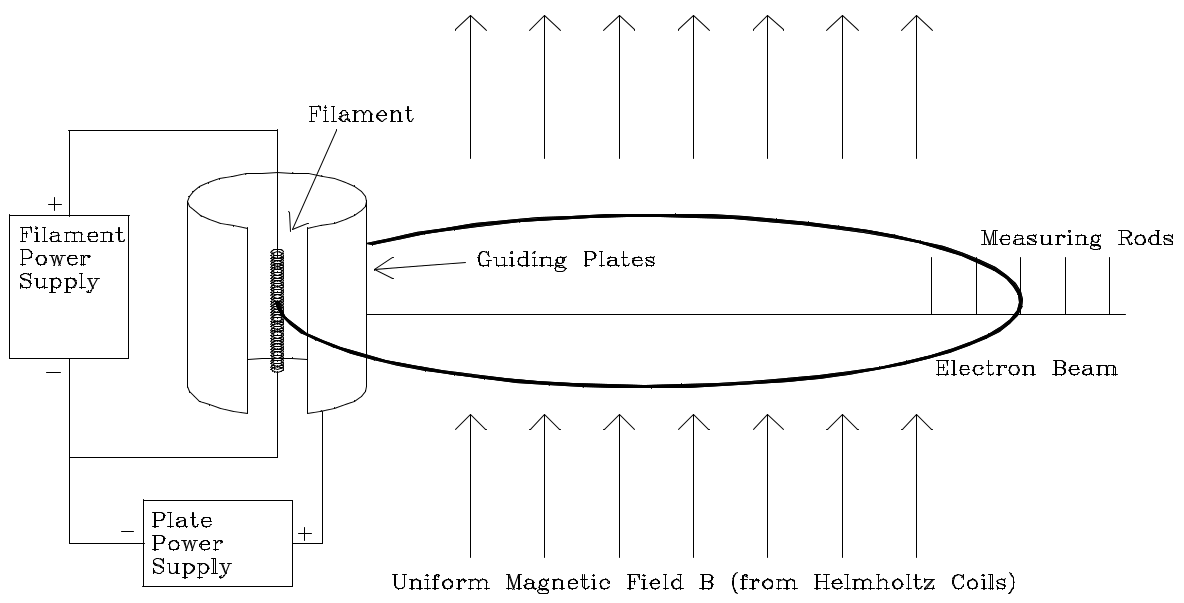
\includegraphics[width=0.6\textwidth]{./Exp5/pic/image1.png}
\caption{Force on a Current-carrying Wire}
\label{fig:force}
\end{figure}

\subsection{Induced EMF in a Coil}
According to Faraday's Law of induction, a changing magnetic flux through a coil induces an EMF (electromagnetic force) $\varepsilon$ given by
\begin{equation}
  \varepsilon=N\frac{\Delta \Phi}{\Delta t}
\end{equation}
where $\Phi = \int \vec{B} \cdot d \vec{A}$ is the flux of magnetic field $B$ through a coil of area $A$ and perpendicular to that area. $N$ is the number of turns in the search coil. For this experiment, the area of the coil is constant and the magnetic field is assumed to be uniform, so the average EMF is given by
\begin{equation}
  \varepsilon= -NA\frac{\Delta B}{\Delta t}
\end{equation}
The negative sign in Faraday's Law comes from the fact  that the EMF induced in the coil acts to oppose any change in the magnetic field. This is summarized as Lenz' Law. It is important to remember that EMF, despite being called a "force" is actually a potential and is measured in volts. Voltage will be induced as the coil enters and leaves magnetic field and its direction will be determined using Lenz' law.

\section{Procedure}
\subsection{Force on a Current-carrying Wire}

The experimental set-up is shown in Figure {\ref{fig:set-up}}. The horizontal magnetic field $B$ is produced in the air gap of a ``C-shaped'' iron electromagnet. The strength of $B$ is determined by the current in the magnet coils $I$, which is supplied by an adjustable low-voltage power supply.\myskip
\begin{figure}[h]
\centering
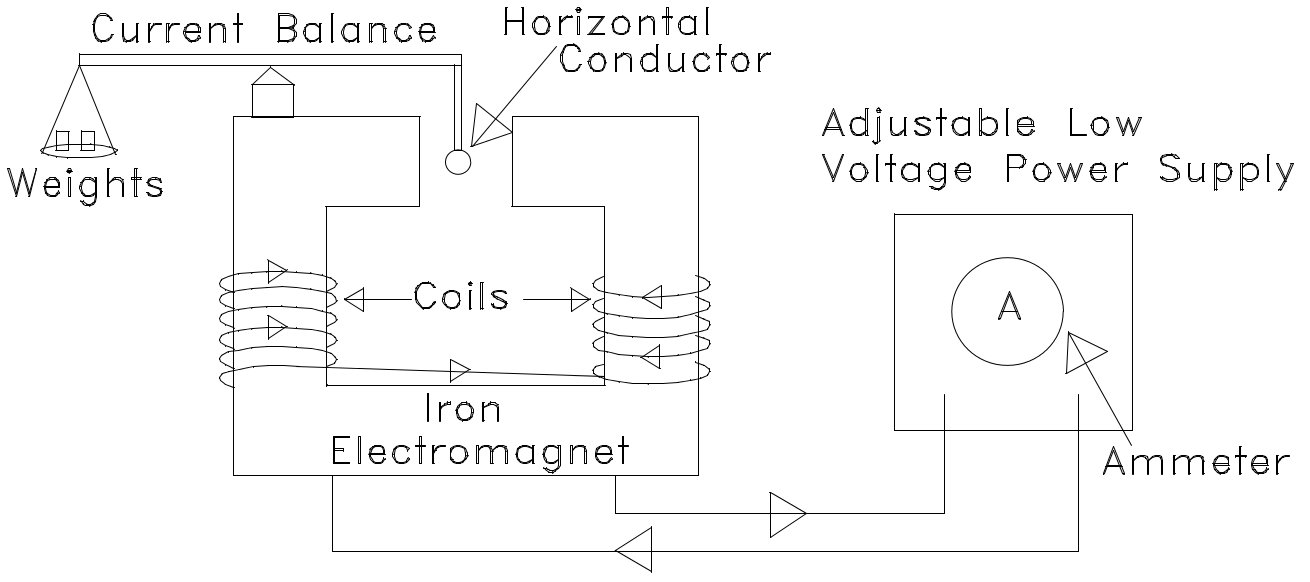
\includegraphics[width=0.8\textwidth]{./Exp5/pic/image2.png}
\caption{Experimental Set-up}
\label{fig:set-up}
\end{figure}

A more detailed drawing of the balance and electro-magnet arrangement is shown in Figure {\ref{fig:measureforce}}.

%\begin{figure}[h]
%\centering
%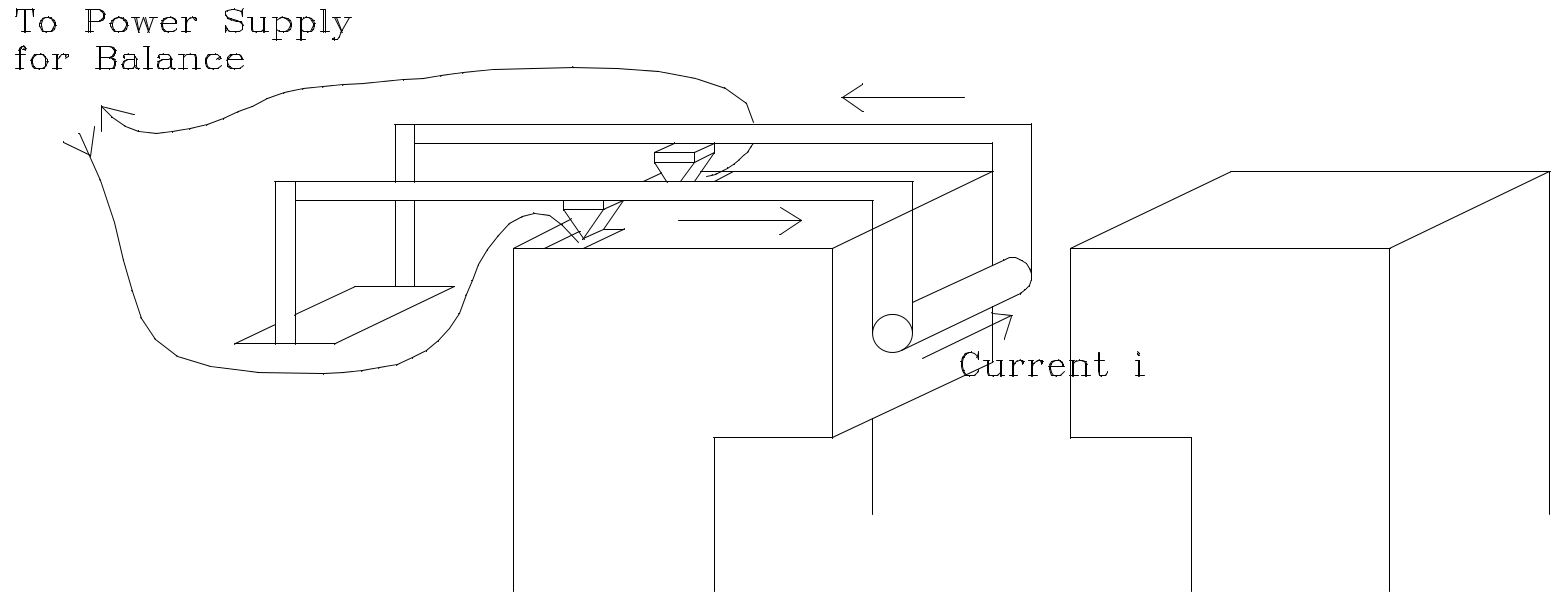
\includegraphics[width=0.8\textwidth]{./Exp5/pic/image3.png}
%\caption{Setup of the Wire and Balance for Force Measurement}
%\label{fig:measureforce}
%\end{figure}

Note that the current $i$ through the horizontal conductor is supplied by a separate power supply. The current balance is constructed out of conducting and insulating materials such that current can enter through one side of the knife-edge fulcrum, flow through one side of the balance arm to the horizontal conductor, and then flow back through the other side of the balance arm and out through the other knife-edge. \myskip

The current $i$ in the balance is provided by the HP E3610A power supply, which can operate either in constant voltage or constant current mode. The voltage dial sets the \emph{maximum voltage} the device will supply to the circuit; the current dial likewise sets the \emph{maximum current}, and if the circuit tries to draw more current, the power supply will reduce the voltage until it reaches whatever value is needed to maintain the maximum current (by $V = IR$). \myskip

To use the power supply in constant current mode, begin with the current dial turned all the way down (counter-clockwise) and the voltage dial turned all the way up (clockwise). Set the range to 3 Amps, and connect the leads to the $+$ and $-$ terminals. You can now set the current to the desired level. Note that the digital meters on the power supply show the \emph{actual} voltage and current being supplied, so you will not normally see any current unless the leads are connected to a complete circuit. (If you want to set the current level without closing the circuit, you can hold in the CC Set button while you turn the current dial.) Once you close the circuit, the voltage adjusts automatically to maintain the constant current level, and the CC (Constant Current) indicator light should be on.

\begin{itemize}
  \item Set the current $I$ through the electromagnet at 5 amperes. Place a small number of weights on the balance and determine the value off $i$ necessary to reach equilibrium. Repeat for at least five different weights.

  \item With Microsoft Excel, plot the weight used to balance the scale vs. the balance current $i$. Include error bars.

  \item Draw a line of best fit and determine the slope with error using LINEST.

  \item From your slope, determine the magnetic field strength $B$ with error.

  \item Repeat the above steps (steps 1-4)  for two other magnet currents $I$ (for a total of three current data sets). You do not need to do error analysis for these measurements, but plot each of your results on the same graph.

  \item Draw a diagram similar to Figure \ref{fig:measureforce} and indicate the directions of $i$, $F$ and $B$ for your setup.

  \item Discuss potential sources of error.
\end{itemize}

\subsection{Induced EMF in a Coil}

\subsection{Experimental Apparatus}

A charge integrator (the Magnetic Field Module shown in Figure {\ref{fig:module}}) is used to measure the $\Delta Q$ produced by the EMF induced in the search coil. A capacitor in the module stores the charge $\Delta Q$, and the voltage across this capacitor (read on the external voltmeter shown) is proportional to $\Delta Q$. Therefore
\begin{equation}
  V=K\Delta Q=K\frac{N}{R}\Delta \Phi
\end{equation}
where $K$ is a constant that depends on the capacitance and gain of the integrator circuit. Instead of trying to calculate a value of $KN / R$ in terms of the components, it is more direct to calibrate the combination of the search coil and the integrator circuit by measuring $V$ for a known $\Delta \Phi$. This known magnetic flux can be created by passing a measured current $I_{\mathrm{sol}}$ through a long air-core solenoid of $n$ turns per meter and with a cross-sectional area of $A_{\mathrm{sol}}$ so that
\begin{equation}
  \Delta \Phi_{\mathrm{sol}}=B_{\mathrm{sol}}A_{\mathrm{sol}}=\mu_{0}nI_{\mathrm{sol}}A_{\mathrm{sol}}
\end{equation}
where $\mu_{0}$ is the permeability of free space ( $\mu_{0} = 4\pi \times 10^{-7}\, \mathrm{T}\cdot  \mathrm{m} / \mathrm{A} $).

\subsection{Procedure}
Connect the apparatus as shown in Figure {\ref{fig:module}}. Turn on the power supply. Before any measurements are made, depress the shorting switch, then release the shorting switch and turn the drift adjust control to minimize the drift in the output voltage as observed on your meter. The shorting switch must be used to discharge the integrating capacitor prior to each measurement. Also, the drift adjust setting should be checked occasionally. If the gain setting on the Magnetic Field Module is changed, the drift adjust control must be reset.\myskip

Magnetic field measurements are made by inserting or removing the search coil from the region containing the field to a field-free region or by leaving the search coil stationary and turning the field on or off.\myskip

Since the magnetic field in the large iron-core electromagnet is much greater than the field in an air-core solenoid, the Magnetic Field Module was designed with two gain settings. In the gain=100 position, the module is 100 times as sensitive as in the gain=1 position. For measuring fields generated by the air-core solenoid, set the gain at 100. For fields generated by the large electromagnet, set the gain at 1.\myskip

Connect the solenoid to the $+$ and $-$ terminals of the HP Power Supply. A three position (on-off-on) reversing switch is part of the solenoid circuit. Flip the switch to one of the on positions and adjust the power supply current such that two amperes is flowing through the solenoid.\myskip

Slide the search coil over the solenoid and, while holding the search coil at the center of the solenoid, discharge the Magnetic Field Module and then turn the current through the solenoid off using the three position switch (or turn the current from off to on). Take several readings and record the voltage on the integrator and the current through the solenoid. Then the result is
\begin{equation}
  V_{\mathrm{sol}}=100\cdot K\cdot \frac{N}{R}\cdot \Delta \Phi_{\mathrm{sol}}=100\cdot K\cdot \frac{N}{R}(\mu_{0}nI_{\mathrm{sol}})A_{\mathrm{sol}}
\label{eq:vsol}
\end{equation}

Now set the gain to 1 on the Magnetic Field Module, and readjust the drift controls. Set the current for the large electromagnet to 5 amps, and use the search coil to measure the resulting $B$. Move the search coil \emph{gently and smoothly} into the region of the magnetic field (do not move the coil hastily as you may damage it by striking against the magnet itself). Record $V_{\mathrm{mag}}$ . The corresponding equation is:
\begin{equation}
  V_{\mathrm{mag}}=K\cdot \frac{N}{R}A_{\mathrm{coil}}B_{\mathrm{mag}}
\label{eq:vmag}
\end{equation}

Combine the results of Eq({\ref{eq:vsol}}) and Eq({\ref{eq:vmag}}) to determine the value of $B$ for the large electromagnet when the current is 5 amps, and then do the same for the other magnet currents of 4, 3, and 2 amps. Compare these values for $B$ with those obtained in Part~I.
